%%%%%%%%%%%%%%%%%%%%%%%
\chapter{データ共有タスク間の順序組合せテストケース抽出手法} \label{chap:5}
本章では,本論文では,統合テストにおける状態遷移間の組合せに着目する,
実践の場においては,S1網羅基準に膨大なテスト工数を要する課題があることから,その対処として経験的なノウハウを基に重要なテストケースを抽出する方法が用いられている\cite{yumoto2006}.
そのひとつの方法として,状態遷移のS1網羅基準のうち,重要な順序組合せを見つけ出す実践的なナレッジとして,状態はタスク内で保持するデータとして実装されることに着目したテストケースの抽出方法がある.
この方法は,保持するデータに対する操作順序が影響することから,データに対するタスクの操作順序パターンを使い,状態遷移の組合せをタスクの順序組合せとしてテストする.
順序組み合わせのテストは,ソフトウェアに変更を加えた場合の変更波及のテストケースとして有効になる.

\newpage
\section{研究の概要} \label{sec:5-1}
\subsection{研究の目的} \label{sec:5-1-1}
前章では,I/O テストデータパターンで単一の$Ta$に対するデータの入出力からテスト条件を網羅的に特定する方法を提案した.
本章では,単一の$Ta$に対するデータの入出力による副作用を確認するテストに着目する.
これは論理的機能構造でのサポートと相互作用に分類されるテスト条件となる.
これらのテスト条件を特定する際のトリガーの一つとして,他処理への反映がある.
他処理への反映をテスト条件に加える目的は,$AS$の一部に変更を加えた場合のその波及の確認が必要となるためである.

ソフトウェアの一部に変更を加えた場合,その変更の波及を探る変更波及解析(Change Impact Analysis)は,実務上の大きな課題である.
産業界において変更にかかる活動は,新規開発よりも大きな割合を占めている.
ゼロから新規にソフトウェアを開発するケースは稀であり,何らかの流用を基に変更を加える開発が主流となっている.
開発方法においてもアジャイルが主流となり,変更の積み重ねによって開発が行われている.
しかし,変更波及を合理的に制御する技術は,ソフトウェア工学とって未完成の分野である\cite{arnold1996software}.
変更の背景は,時代と共に課題を難しくしている.
ソフトウェアの多様化と複雑化,再利用範囲の増大などから変更波及の範囲が拡大し,かつ安易な変更による弊害など課題が山積している.
これらの課題に対してソフトウェア工学は十分な解を提供できていない状況にある\cite{li2013survey}.
本章では,状態遷移を持つソフトウェアにおいて,変更波及がデータベースや外部変数などの保持データを介して生ずる場合のテストについて考える.
課題の一つは,網羅基準である.データフローテストの全使用法(AU法)\cite{beiz90}を基にして,変更波及のテスト網羅基準を波及全使用法(Impact Data All Used:IDAU)として提案する.
もう一つの課題は,IDAU法を満たす具体的な変更波及のテストケースの抽出方法である.変更波及のテストの設計手法として,順序組合せテストを提案する.
最後に,ここで提案するIDAU法のコストの評価,すなわちテストケースの数を従来技法である状態遷移テストのS1網羅基準と比較をして考察を行い,提案する方法が合理的であることを示す.


\newpage
\section{変更波及とその解析}
本節では,提案する網羅基準やテスト設計手法の前提となる,システムの構成と変更について定義し,変更波及をテストする課題について詳細を示す.

\subsection{変更と変更波及}
$AS$に対して,何らかの変更を加える場合について考える.
変更には,なんらかの意図があり,$AS$が持つ機能の変更であったり,不具合に対する変更や,性能や保守性の改善のためのリファクタリングであったりする.
本論文では,変更の意図については取り扱わず,$AS$の構成要素(タスク,状態,保持データ)に対する具体的な変更について考える.ただし,テスト実行するためには,タスクを動かすことが必要となる.そのため,以降の議論はタスクに焦点を絞る.%1-1対応

ひとつの変更$Q$について考える.
変更$Q$は,タスク群$Ta$のあるタスク$Ta_i$に対して行われたとする.
変更$Q$は,コードの削除や追加を含み,その結果$Ta_i$の版$R$が$R+1$に変更される.
この変更の結果を$Ta^{R}_i$から$Ta^{R+1}_i$とする.

変更$Q$の波及には,3つのケースが考えられる.
\begin{enumerate}
  \item 変更波及が無い場合.(リファクタリングに相当)
  \item 変更波及が他のタスクへ波及しない場合.%3-7対応
  \item 変更波及が他のタスクへ波及する場合.
\end{enumerate}

3.の変更波及は,タスク間の参照が図\ref{fig:fig-2}に示すように状態と保持データに限られるならば,該当する状態や保持データの参照を介した範囲が限られると考えられる.
本論文では,この考え方から波及を受けるタスクを特定し,その合理的なテスト設計について論じる.


%−−−-図2を入れる

\begin{figure}[b]
\begin{center}
\includegraphics[scale=0.5]{./image/fig-2.png}
\end{center}
\caption{変更タスクと変更波及}
\label{fig:fig-2}
\end{figure}

変更波及,あるいはその解析(Change Impact Analysis)に関する研究は古くから行われている.プロダクトラインやUML図面群を基に依存関係生成モデルを用いて波及解析を行う研究がある\cite{gomaa2005designing}\cite{2008kotani}\cite{briand2003impact}
タスク内のデータフローを基に変更波及を詳細に解析した研究がある\cite{campbell1990}.
データベースなど保有データを基に変更波及解析を行う研究も行われている\cite{maule2008impact}\cite{2011ogawa}.
一方,状態と状態遷移はマルコフ過程として実装されているので,過去の状態が未来の状態に影響しない.状態遷移に関する波及解析の研究は見当たらないのはそのためだと推測する.%3-8対応
\cite{LSOF}
\cite{kang1990feature}
\subsection{状態と変更波及のテスト}
変更波及は,保持データを介して波及タスクへ伝達する.状態や状態遷移自身は変更波及に関与しないが,変更波及のテストにおいて与えるデータの順序において状態を考慮する必要が生じる.

保持データの構成について考える.その要素を$Ds=\{Ds_1,Ds_2,\cdots,Ds_j,\cdots,Ds_d\}$とし,変更波及を受ける保持データの要素を$Ds_j$とする.
保持データに対する操作は,データのライフサイクルである「生成:C」「参照:R」「更新:U」「削除:D」を記したCRUD図で定義する.
$Ds_j$を介して変更波及が生ずるのは,変更タスク$Ta_i$において「生成:C」あるいは「更新:U」が行われ,他のタスクで「参照:R」が行われた場合に波及タスクとなる.

保持データのライフサイクル上の「生成:C」「参照:R」「更新:U」「削除:D」などの操作は,無条件に行われるのではなく,操作するタスクの制御フローに沿って行われる.
制御フローは,2階層として捉えることができる.上位の制御フローはタスクの実行順序により決定される大きな制御の流れに相当する.
個々のタスク内の制御フローが下位にあたる.個々のデータ参照実行文はその制御フロー上の条件文で実行が決定される.
条件にはタスクへの入力,保持データ,状態が含まれる.

変更波及を確認するには,変更が波及した保持データを参照するデータフローに沿ってテストを設計することになる.
このデータフローを決定するのは,関係するタスクの実行順序とタスク内の制御フローであり,その制御フローを決定する際に状態が影響する.
状態による制御が想定通りに行われない欠陥は,タスクの実行順序により決定される大きな制御の流れの判断のための状態の確認を,タスク実行のあるタイミングでのみ行っていることが原因となる.%1-2対応による追記
よって,実際のテスト実行においては状態を考慮する必要が生ずる.

\subsection{変更波及テストの網羅基準}

テストにおける網羅基準については,その強度を含め制御フローとデータフローの観点から研究が行われ体系が作られている\cite{beiz90}.
最も弱い網羅基準は制御フローのみに着目した実行文網羅,次が分岐網羅であり,最も強い網羅基準はデータフローを含めた全パス網羅(All Paths)である.%3-9
全パステストは,すべての分岐の積であり現実的には実現不可能のため,全使用法(All Uses)が推奨されている\cite{beiz90}.

変更波及をテストする場合,波及に関与するデータに着目し,そのデータフローテストを行う.
一般的な全使用法は「データを定義したすべての場所から始まり,データを使用するすべての場所に至るまでのパスセグメントを最低限1つを含むテストケース」と定義されている\cite{beiz90}.
この定義を変更タスクと波及タスクとの関係に置き換え「変更タスクにおいてデータの生成および更新があるデータを使用するすべてのタスク(波及タスク)を2つのタスクを実行するまでに経由するルートにかかわらず最低限1つ含むテストケース」とし,波及全使用法とする.

\newpage
\section{順序組合せによるテストケース抽出法} \label{sec:5-2}
本節では,状態遷移テスト設計におけるS1 網羅基準 ではテストケース数が爆発するが,S0網羅基準では漏れが 生じるという課題を解決する手法として順序組合せテストを提案する.

\subsection{入力情報}
 一般的にテストケース抽出のために必要な入力情報をテストベースと呼ぶ\cite{Demarco}.
提案手法に必要なテストベースは DFD,ER 図,CRUD 図である.以下,DFD,ER 図,CRUD 図を簡潔に説明する.

\begin{itemize}

\item DFD(データフローダイアグラム)

DFDはシステムにおけるデータの流れを表現した有向グラフであり,要求分析において用いられている.
DFDはデータ指向設計の要として用いられ,オブジェクト指向設計においても抽象化する前段階として実践の場で用いられている.

DFDは,最上位のコンテキストレベルから階層として詳細化され,各階層は1枚以上のDFDから成る\cite{Demarco}.
テストベースとして用いる場合,テストの範囲はDFDで与えられるとする.DFDの階層が下がると単体テストとなり,上がると統合テストとなる.

DFDはノードとエッジからなる.
ノードは3種類の要素である$N$個のタスク(プロセス)$Ta$と,$M$個の保持データ(データストア)$Ds$と,$L$個の源泉(外部エンティティ)$So$から構成されている.%3-11対応
3種類の要素を一意に特定する際は$Ta_i$,$Ds_j$,$So_k$と表記する.

エッジは,ノードからノードへのつながりを有向線分で表記している.エッジはデータの流れを表しており,制御の流れは表していない.
エッジの特定は,起点ノードと終点ノードを用いて行う.
ある特定のタスクからデータストアへの入力がある場合のエッジの特定は,$Ta_i/Ds_j$となり,源泉から出力してタスクで処理をする場合は,$So_k/Ta_i$と表す.%3-12対応

\item ER図

ER図はシステムにおけるエンティティ間の関係を示す図であり,UMLのクラス図に対応している.
DFDでは表現できないエンティティの詳細化やエンティティ間の関係について示しており,DFDと共に用いられている.

ここでは,DFDのデータストア$Ds_j$が持つエンティティと,CRUD図の対応から,後述する拡張CRUD図を作成するために用いる.
よって,テストベースとしては,システムすべてのER図を必要とするものではない.

\item CRUD図

CRUD図とは,タスク$Ta_i$からデータストア$Ds_j$への$C$:生成,$U$:更新,$R$:参照,$Ds$:削除の操作を表した図である\cite{Politano}.
CRUD図から,DFDとER図では表現されていないタスクのエンティティへの操作を知ることができる.

本論文では,タスクがデータストアに対して行う操作を特定するためにCRUD図を用いる.
タスク$Ta_i$のデータストア$Ds_j$に対する操作が$U$:更新であればタスクによる操作はエッジを介した操作として$Ta_i/Ds_jU$と表記する.
ただし,タスクが操作するデータストアが1つだけの場合は,$Ta_iU$といった省略した表記を使う.
\end{itemize}

\subsection{順序組合せテストの概要} \label{sec:5-2-1}
提案する手法は,2タスク間の順序組合せを対象とする.
2タスク間の順序組合せの抽出は以下のルールを適用する.
\begin{itemize}

\item ルール1:変更タスクの特定
%20170305
%対象とするDFDにおけるタスクにおいて,源泉$So$からの入力エッジがあり,かつデータストア$Ds$へ出力エッジを持つタスクを選択し順序組合せの変更タスク群$P\{Ta\}$とする.

対象とするDFD内の変更タスクのうち,データストア$Ds$へ出力エッジを持つタスクを選択し,順序組合せの変更タスク群$P\{Ta\}$とする.%3-14対応
変更タスク群からの出力するデータストア群を$P\{Ds\}$とする.

\item ルール2:波及タスクの特定

ルール1で求めた$P\{Ds\}$からの入力エッジを持つタスクを波及タスク群$S\{Ta\}$として特定する.

\item ルール3:順序組合せテストケースの抽出

拡張CRUD図を基に変更タスク群$P\{Ta\}$とそのデータストア群$P\{Ds\}$を介する波及タスク群$S\{Ta\}$を組合せ,順序組合せのテストケースとする.
\end{itemize}

以降からは,順序組合せを抽出してテストケースとするまでの実施手順を詳細に説明する.

\subsection{ルール1:変更タスクの特定}
% Table generated by Excel2LaTeX from sheet 'Sheet1'
\begin{table}[t]
\caption{拡張CRUD図}
\label{CRUDIO}
\begin{center}
\begin{tabular}{r|r|r|r|r|r|r}
\multicolumn{1}{c|}{タスク} & \multicolumn{3}{c|}{データストア} & \multicolumn{3}{c}{源泉} \\
\cline{2-7}\multicolumn{1}{c|}{} & $Ds_1$ & $...$ & $Ds_j$ & $So_1$ & $...$ & $So_k$ \\
\hline
\hline
$Ta_1$ &   &   &   &   &   &  \\
\hline
$...$ &   &   &   &   &   &  \\
\hline
$Ta_i$ &   &   &   &   &   &  \\
    \hline
\end{tabular}%
%\halflineskip
\end{center}
\end{table}

ルール1を用いて変更タスクとそのデータストアを特定し,拡張CRUD図の変更タスク部分を作成する.


拡張CRUD図とは,テストベースとして与えられたDFD,ER図,CRUD図から$P\{Ta\}$の各$Ta_i$と関連する$So_k$,そして$P\{Ds\}$となる$Ds_j$の関係を追加して作成したものである.
表 ~\ref{CRUDIO}に拡張CRUD図の表記を示す.
拡張CRUD図のデータストアに対する情報は$C$,$U$,$R$,$D$のいづれか,または組合せか空白である.
源泉に対する情報は$In$か$Out$,または組合せか空白である.
空白は関係が無いことを示す.

\begin{enumerate}
\item 源泉からの入力エッジを持つ変更タスクの特定

%状態について記載するように変更した.補集合で表現するようにした
%元のストーリーである、外部入力があるタスクはそのままにして、更に抽出する要素として、「変更のある」を追加した.
テストケースは,外部からのテスト対象への入力から,外部への出力結果を確認するものであるため,テスト入力とテスト結果のペアで構成されている.
そこで,テスト対象範囲の外からの入力,即ち$So_k$からの入力エッジを持つ$Ta_i$を見つける必要がある.
この特性を持ったタスクのうち,さらに変更のあるタスク群を変更タスクの集合となる$P\{Ta\}$候補とする.
変更が特定の状態でのみ起こり得る場合は,タスクの後に変更が起きる状態を[$St_l$]と記載する.
%上記は追加部分

\item データストアへの出力エッジを持つタスク特定

$Ta_i$から$Ds_j$への出力エッジは,$C$か$U$か$D$の操作を行うことを意味する.CRUD図から該当する出力エッジを持つ$Ta_i$を選択する.
$P\{Ts\}$候補の中から,該当する$Ta_i$を選び,変更タスク群$P\{Ta\}$を確定する.

\item 中間の拡張CRUD図作成

拡張CRUD図には,変更タスク群$P\{Ta\}$に該当する$So_k$から$Ta_i$への入力($In$),もしくは$Ta_i$から$So_k$への出力($Out$)の情報を付加する.
特定した$Ta_i$に対して,入力となる$So_k$に$In$を記入し,$Ds_j$についてはCRUD図を参照して$C$か$U$か$D$かその組合せかを記入する.
中間の拡張CRUD図として例示した表 ~\ref{CRUDIO2}では,3つの源泉$\{So_1,So_2,So_3\}$と3つのデータストア$\{Ds_1,Ds_2,Ds_3\}$があり,2つのタスク$\{Ta_1[St_1],Ta_3[St_1]\}$が変更タスクである.
この段階で作成する拡張CRUD図は,作業途中のものである.

\end{enumerate}


% Table generated by Excel2LaTeX from sheet 'Sheet1'
\begin{table}[t]
  \centering
  \caption{中間の拡張CRUD図の例}
    \begin{tabular}{r|r|r|r|r|r|r}
    \multicolumn{1}{c|}{タスク} & \multicolumn{3}{c|}{データストア} & \multicolumn{3}{c}{源泉} \\
\cline{2-7}    \multicolumn{1}{c|}{} & $Ds_1$ & $Ds_2$ & $Ds_3$ & $So_1$ & $So_2$ & $So_3$ \\
    \hline
    \hline
    $Ta_1[St_1]$ & $CU$ &   &   & $In$ &   &  \\
    \hline
    $Ta_3[St_1]$ &   & $C$ &   & $In$ &   &  \\
    \hline
    \end{tabular}%
 \label{CRUDIO2}
\end{table}%



\subsection{ルール2:波及タスクの特定}
ルール2を用いて波及タスク群を特定し,拡張CRUD図へ波及タスク部分を追加し図を完成させる.

\begin{enumerate}
\item データストアを介した波及タスク特定
%\item データストアを介した\end{enumerate}波及タスク特定
%なぜ\UTF{2613}と−がテストしなくてよいかということを追記した.
先に作成した中間の拡張図から変更タスクの操作が$C$か$U$か$D$であるデータストアに着目する.
着目したデータストアに対してエッジを持つタスクが波及タスクの候補となる.
波及タスクとして選択するタスクは表 ~\ref{table:3}に示す表の○印の組合せに該当するタスクである.
\begin{table}[h]
\caption{タスク間のデータ共有の組合せパターン}
\label{table:3}
\begin{center}
\begin{tabular}{c|c||c|c|c|c}
\hline
\multicolumn{2}{c||}{}& \multicolumn{4}{c}{$P\{Ta\}$}\\
\multicolumn{2}{c||}{}& C & R & U& D\\
\hline\hline
$S\{Ta\}$&C&×&×&×&◯\\
\cline{2-6}
&R&◯&-&◯& -\\
\cline{2-6}
&U&◯&-&◯&×\\
\cline{2-6}
&D&◯&- &◯&×\\
\hline
\end{tabular}
%\halflineskip
\end{center}
\end{table}
波及タスクは, C:生成,U:更新,D:削除を選択する.
”-”をつけた組合せは,データストアを介した影響が生じないため,組合せテストの対象としない.
”×”をつけた組合せは仕様上有り得ない組合せであり,ありえないことの確認は,順序組合せを網羅しなくともよいため,組合せテストの対象としない.

着目したデータストアに対してエッジを持つタスクが波及タスクのうち,源泉に出力エッジを持つタスクを波及タスクとして特定する.
特定した波及タスクを拡張CRUD図に追記し完成させる.
\item 拡張CRUD図の完成
波及タスク候補のうち,源泉に出力エッジを持つタスクを波及タスクとして特定する.
波及タスクの特性をDFDより読み取り,特定する.
特定した波及タスクを拡張CRUD図に追記し完成させる.
完成させた拡張CRUD図の例を表~\ref{excrud}に示す.
この例では,
データストア$Ds_1$から源泉$So_2$への流れをタスク$Ta_2[St_1]$が行い,
データストア$Ds_2$から源泉$So_3$への流れをタスク$Ta_5[St_1]$が行っていることを示している.
\end{enumerate}
% Table generated by Excel2LaTeX from sheet 'Sheet1'
\begin{table}[t]
  \centering
  \caption{完成した拡張CRUD図の例}
    \begin{tabular}{r|r|r|r|r|r|r}
    \multicolumn{1}{c|}{タスク} & \multicolumn{3}{c|}{データストア} & \multicolumn{3}{c}{源泉} \\
\cline{2-7}    \multicolumn{1}{c|}{} & $Ds_1$ & $Ds_2$ & $Ds_3$ & $So_1$ & $So_2$ & $So_3$ \\
    \hline
    \hline
    $Ta_1[St_1]$ & $CU$ &   &   & $In$ &   &  \\
    \hline
    $Ta_3[St_1]$ &   & $C$ &   & $In$ &   &  \\
    \hline
    $Ta_2[St_1]$ & $R$ &   &   &   & $Out$ &  \\
    \hline
    $Ta_5[St_1]$ &   & $R$U &   &   &   & $Out$ \\
    \end{tabular}%
  \label{excrud}%
\end{table}%

\subsection{ルール3:順序組合せテストケースの抽出}
\begin{enumerate}
\item 変更タスクと波及タスクの組合せを抽出

拡張CRUD図から変更タスクを選ぶ.
先に作成した拡張CRUD図の例(表~\ref{excrud}を参照)であれば,$Ta_1[St_1],Ta_3[St_1]$である.
次に変更タスクが操作しているデータストアと,それを操作している波及タスクを対応付ける.
例では,$Ta_1[St_1]  \xrightarrow[Ds_1]{} Ta_2[St_1]$と$Ta_3[St_1]  \xrightarrow[Ds_2]{}  Ta_5[St_1]$である.
\item データストアに対する操作の組合せ

操作の組合せとは変更タスクと波及タスクの操作の組合せである.
%表 ~\ref{excrud}の例であれば,変更タスクのデータストアに対する操作,$Ta_1$は$Ds_1$に対して$CU$の操作を行っている.%3-21対応
表 ~\ref{excrud}の例であれば,変更タスクのデータストアに対する操作である$Ta_1$は,$Ds_1$に対して$C$と$U$の操作を行っている.
波及タスク$Ta_2$の操作は$R$である.
組合せは$C  \rightarrow R$と$U  \rightarrow R$となる.
変更タスクと波及タスク間に介在するデータストアが1つであれば$\xrightarrow[Ds_1]{}$を省略して$\rightarrow$で表してもよい.
また変更の発生条件となる状態が1つであれは,$[St_1]$を省略してもよい.
表~\ref{excrud}の例における全組合せは,$Ta_1C \rightarrow Ta_2R$,$Ta_1U \rightarrow Ta_2R$,$Ta_3C \rightarrow Ta_2R$,$Ta_3C \rightarrow Ta_2U$の4個である.

\item テストケース表の完成

変更タスクと波及タスクの操作の組合せをテストケースとしてまとめる.表 ~\ref{TCLISTSAMPLE}にその例を示す.概要の部分は,当該組合せが持つ入力の条件や出力の特性を仕様から抜き出して記載する.
\end{enumerate}

% Table generated by Excel2LaTeX from sheet 'Sheet1'
\begin{table}[t]
  \centering
  \caption{順序組合せテストによる論理的テストケースの例}
    \begin{tabular}{l|l|l}
    No & 論理的テストケース & 順序組合せ \\
    \hline
    1 & 概要 & $Ta_1C \rightarrow Ta_2R$ \\
    \hline
    2 & 概要 & $Ta_1U \rightarrow Ta_2R$ \\
    \hline
    3 & 概要 & $Ta_3C \rightarrow Ta_2R$ \\
    \hline
    4 & 概要 & $Ta_3C \rightarrow Ta_2U$ \\
    \hline
    \end{tabular}%
\label{TCLISTSAMPLE}
\end{table}%

以上の手順で,順序組合せテストに必要なテストケースを抽出する.
ここで用いたテストケースとは,ISTQBの定義による論理的テストケースに相当する\cite{ISTQB}.

具体的な値や期待結果,該当の処理までの状態を遷移させていく手順まで定義した記述を具体的テストケースと呼ぶが,本論文では扱わない.

\newpage
\section{評価実験} \label{sec:5-3}
\subsection{実験の概要} \label{sec:5-3-1}

本節では,旅行代理店向けフライト予約システムの仕様を用いて,3章で述べた実施手順を適用し,順序組合せが抽出できることを確認する.

\subsection{題材の概要}
フライト予約システムの概要を以下に示す.
%・フライト予約システムの概要を説明する\\
\begin{figure}[h]% fig.1
\setbox0\vbox{%
{\small
%{\footnotesize
\hbox{\verb/<フライト予約システム概要>/}
\hbox{\verb/・旅行代理店用に開発したフライト予約サーバにインターネット経由で/}
\hbox{\verb/ アクセスできる専用のクライアントアプリケーション./}
\hbox{\verb/・旅行代理店の窓口での利用を想定しており,ユーザ認証されたユーザ/}
\hbox{\verb/ のみ利用可能である./}
\hbox{\verb/・旅行代理店の窓口数(クライアント数)は50としており,同時に予約/}
\hbox{\verb/ 処理を行うことができる./}
\hbox{\verb/・旅行代理店にて取り扱う全ての航空会社の飛行機の予約が可能で/}
\hbox{\verb/ ある./}
\hbox{\verb/・本システムは,フライト予約サーバを仲介して複数の航空会社のシス/}
\hbox{\verb/ テムと同期をする./}
\hbox{\verb/・チケット情報や残チケット数は同期することで最新に更新される./}
\hbox{\verb/・フライトの新規予約、予約内容の更新,削除が可能である.更新と/}
\hbox{\verb/ 削除は新規予約したユーザのみ可能である./}
\hbox{\verb/・以下はシステム範囲外/}
\hbox{\verb/ -チケット代金の決済(別システムと連携して行うため)./}
\hbox{\verb/ -マスタ情報設定(他システムとの共用マスタ設定アプリケーションが/}
\hbox{\verb/  あるため)./}
}
}
\begin{center}
\fbox{\box0}
\end{center}
\caption{フライト予約システムの概要}
\label{OVSPEC}
\end{figure}

\begin{figure*}[tb] %ER図とDFD.最初と最後に*を入れると1段で入る
\begin{center}
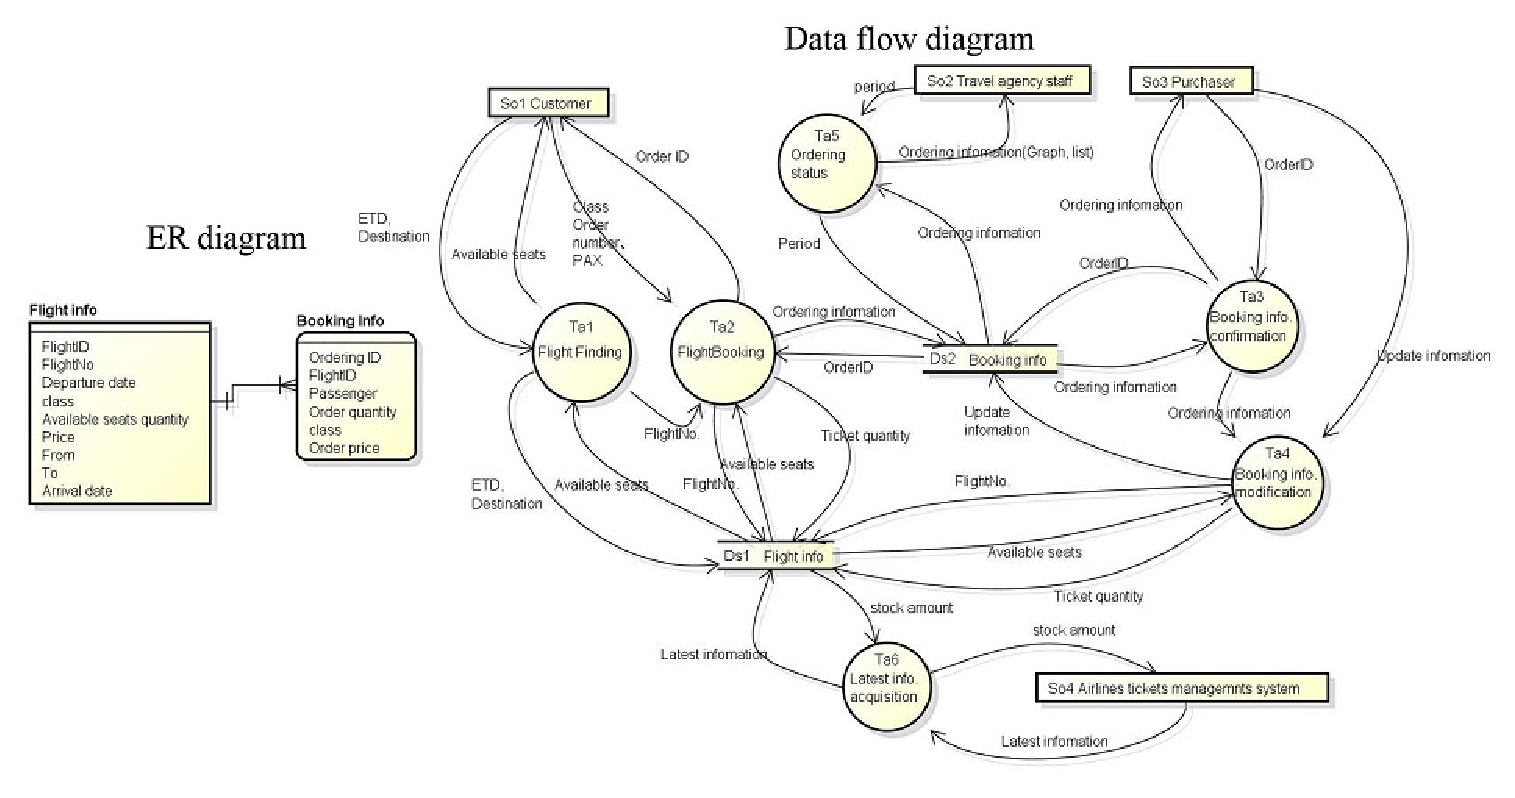
\includegraphics[scale=0.68]{./image/dfdanderd.eps}
\end{center}
\caption{新規フライト予約のデータ設計(一部分)}
\label{fig:DFD}
\end{figure*}

題材となるフライト予約システムの仕様は,本研究の一環として評価実験の際に題材として使っているものである\cite{yumoto2015ICST}\cite{yumoto2016ICST}.
テスト対象の分析と,テストケース設計に関する用語は,国際標準であるISO/IEC/IEEE29119の定義に従い,テスト対象の論理的なサブセットをフィーチャーセットと呼ぶ\cite{ISO29119}.%3-22対応
本論文では,表~\ref{Featurelist}の新規フライト予約を,変更が入ったフィーチャーセットとする.


新規フライト予約からテストケースを抽出するための前提として用意した仕様は,新規フライト予約に関連するDFDとER図(図~\ref{fig:DFD}),CRUD図(表~\ref{CRUD})とする.
DFDに含まれるタスク数 $N$は6,データストア数$M$は2,源泉数$L$は4である.

\begin{table}[t]
\caption{フライト予約システムのフィーチャーセット一覧}
\label{Featurelist}
\begin{center}
\begin{tabular}{l|l}
\hline
テストアイテム&フィーチャーセット
\\
\hline\hline
フライト予約システム&メニュー\\
\cline{2-2}
&ログイン\\
\cline{2-2}
&新規フライト予約\\
\cline{2-2}
&予約変更 \&\\
&キャンセル\\
\cline{2-2}
&予約一覧\\
\cline{2-2}
&予約グラフ\\
\cline{2-2}
&同期処理\\
\hline
\end{tabular}
%\halflineskip
\end{center}
\end{table}

\begin{table}[t]
\caption{フライト予約システムのCRUD図}
\label{CRUD}
\begin{center}
{\footnotesize
\begin{tabular}{p{1.7 cm}|c|p{1.5 cm}||p{1 cm}|p{1cm}}
\hline
フィーチャーセット&\multicolumn{2}{c||}{タスク}&\multicolumn{2}{c}{エンティティ}\\
&\multicolumn{2}{c||}{}&$Ds_1$&$Ds_2$\\
&\multicolumn{2}{c||}{}&Flight info.&Booking info.\\
\cline{4-5}
\hline\hline
新規フライト予約&$Ta_1$&フライト検索&R&\\
\cline{2-5}
&$Ta_2$&フライト登録&RU&C\\
\hline
予約変更&$Ta_3$&予約情報確認&&R\\
%Booking cancellation&&&&\\
\cline{2-5}
キャンセル&$Ta_4$&予約情報修正&RU&UD\\
\hline
\shortstack{予約リスト\\予約グラフ}&$Ta_5$&注文状況&&R\\
\hline
\cline{2-5}
同期処理&$Ta_6$&最新情報取得&CU&\\
\hline
\end{tabular}
}
%\halflineskip
\end{center}
\end{table}%

%-----------

\subsection{ルール1:変更タスクの特定}
テストベースであるDFDに含まれるタスク数$N$は6であるが,変更が入った新規フライト予約の変更タスクは,表~\ref{CRUD}のCRUD図を確認するとフライト検索$Ta_1$とフライト予約$Ta_2$であることがわかる.
図~\ref{fig:DFD}から,$Ta_1$と$Ta_2$の外部入力を確認する.
$Ta_1$は,Customer$So_1$からETDとDestinationを外部入力し,$Ta_2$は,Customer$So_1$からFlightNo,Cl$AS$s,Order number,PAXを外部入力している.

続いて,$Ta_1$と$Ta_2$の内部出力を確認する.
$Ta_1$はFlight info$Ds_1$に対して検索条件を与えているのみで内部入力はしていないため,変更タスク群$P\{Ta\}$からは除外する.
$Ta_2$がFlight info$Ds_1$で$U$,Booking info$Ds_2$で$C$を行っていることが表~\ref{CRUD}から読み取れる.
これらから,拡張CRUD図(表~\ref{ECRUD1})を作る.
表~\ref{ECRUD1}から,ルール1に適合する$Ta_2/Ds_1U$,$Ta_2/Ds_2C$を特定できる.

\begin{table}[t]
\caption{フライト予約システムの中間拡張CRUD図}
\label{ECRUD1}
\begin{center}
\begin{tabular}{c||c|c||c|c|c|c}
\hline
タスク&\multicolumn{2}{c||}{データストア}&\multicolumn{4}{c}{源泉}\\
&$Ds_1$&$Ds_2$&$So_1$&$So_2$&$So_3$&$So_4$\\
\hline\hline
$Ta_1$&&&&&&\\
\hline
$Ta_2$&$U$&$C$&$In$&&&\\
\hline
\end{tabular}
%\halflineskip
\end{center}
\end{table}%

\subsection{ルール2:波及タスクの特定}
ルール2にて波及タスク群$S\{Ta\}$を抽出するために,タスクの外部出力を図~\ref{fig:DFD}のDFDから調べる.
$P\{Ds\}$に含まれる$Ds_1$と$Ds_2$とエッジを持ち,かつ$So$へ出力するタスク群が$S\{Ta\}$候補である.
図~\ref{fig:DFD}では,全てのタスクが$Ds_1$および$Ds_2$からのエッジを持つ.
しかし,$So$への出力に着目すると,$Ta_4$は該当するエッジがないため,$S\{Ta\}$候補には入らない.

$S\{Ta\}$候補のうち、表~\ref{table:3}の○がつく組合せに相当する$Ta_i$が,ルール2で特定したタスクとなる.
本章の例の場合,$P\{Ta\}$での操作は,$C$と$U$であるため,$S\{Ta\}$候補の中で$C$の操作をする$Ta_i$以外は全てルール2で特定したタスクとなる.

これらに該当する$Ta_i$と$Ds$へのCRUD操作,そして$So$への$Out$を追記し,表~\ref{ECRUD2}を完成させる.

\begin{table}[t]
\caption{フライト予約システムの拡張CRUD図}
\label{ECRUD2}
\begin{center}
\begin{tabular}{c||c|c||c|c|c|c}
\hline
タスク&\multicolumn{2}{c||}{データストア}&\multicolumn{4}{c}{源泉}\\
&$Ds_1$&$Ds_2$&$So_1$&$So_2$&$So_3$&$So_4$\\
\hline\hline
$Ta_1$&$R$&&$Out$&&&\\
\hline
$Ta_2$&$RU$&$C$&$InOut$&&&\\
\hline
$Ta_3$&&$R$&&&$Out$&\\
\hline
$Ta_5$&&$R$&&$Out$&&\\
\hline
$Ta_6$&$CU$&&&&&$Out$\\
\hline
\end{tabular}
%\halflineskip
\end{center} 
\end{table}%

\subsection{ルール3:手順 順序組合せテストケースの抽出}
表~\ref{ECRUD2}の拡張 CRUD 図から変更タスクと波及タスクの組合せを抽出する.
抽出した変更タスクと波及タスクの組合せに対して,データストアに対する操作を明記したものは以下のとおりとなる.
\begin{itemize}
\item $Ta_2/Ds_1U  \xrightarrow[Ds_1]{} Ta_1R$\\
\item $Ta_2/Ds_1U  \xrightarrow[Ds_1]{} Ta_2/Ds_1U$\\
\item $Ta_2/Ds_1U  \xrightarrow[Ds_1]{} Ta_6U$\\
\item $Ta_2/Ds_2C  \xrightarrow[Ds_2]{} Ta_3R$\\
\item $Ta_2/Ds_2C  \xrightarrow[Ds_2]{} Ta_5R$\\
\end{itemize}
これらの変更タスクと波及タスクの操作の順序組合せがテストケースとなる.
抽出した順序組合せが持つ入力の条件や出力の特性を仕様から抜き出して論理的テストケースとしてまとめる.
表~\ref{TCLIST2}に論理的テストケースとしてまとめた結果を示す.
\begin{table}[h]
\footnotesize
\caption{順序組合せテストによる論理的テストケース}
\label{TCLIST2}
\begin{center}
%\begin{tabular}{c|p{1 cm}|p{3.5 cm}|p{1.5 cm}}
\begin{tabular}{c|p{3 cm}|p{2.1 cm}}
\multicolumn{3}{l}{新規フライト予約}\\
\hline
No&論理的テストケース&順序組合せ\\
\hline\hline
1&フライト予約後の空き情報問合せによる同一フライトの参照&$Ta_2/Ds_1U  \xrightarrow[Ds_1]{} Ta_1R$\\
\hline
2&フライト予約後の再度同一フライトの予約&$Ta_2/Ds_1U  \xrightarrow[Ds_1]{} Ta_2/Ds_1U$\\
\hline
3&フライト予約後の同期処理によって最新のチケット残数の計算&$Ta_2/Ds_1U  \xrightarrow[Ds_1]{} Ta_6U$\\
\hline
4&既存注文開く画面での予約したフライトの参照&$Ta_2/Ds_2C  \xrightarrow[Ds_2]{} Ta_3R$\\
\hline
5&注文件数グラフ・注文履歴の一覧への新規予約フライト予約の反映&$Ta_2/Ds_2C  \xrightarrow[Ds_2]{} Ta_5R$\\
\hline
\end{tabular}
%\halflineskip
\end{center}
\end{table}

\subsection{順序組合せテストの適用評価} \label{sec:5-2-2}
\begin{figure}[h]
\begin{center}
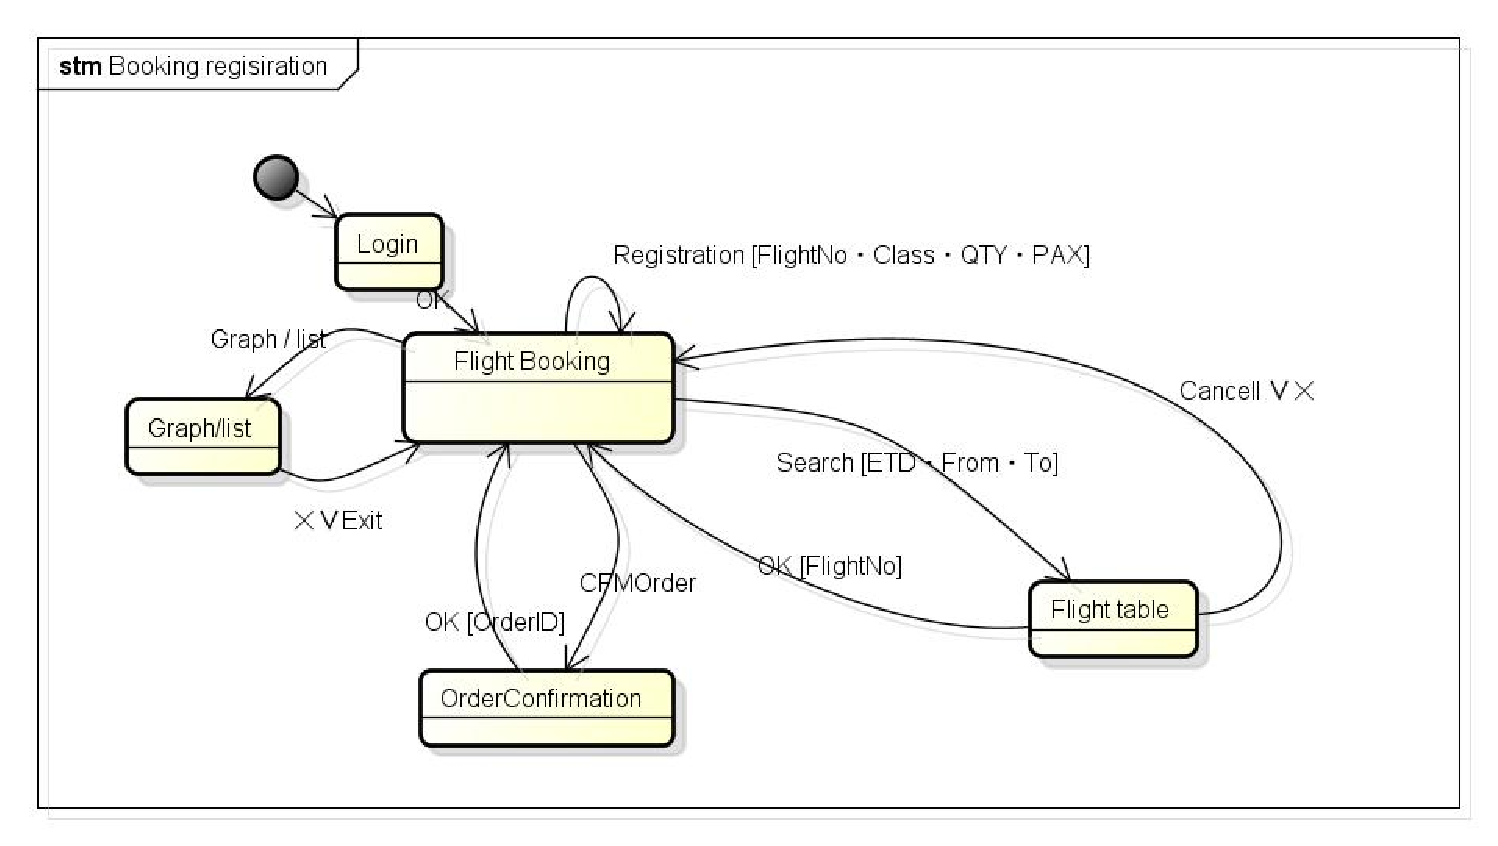
\includegraphics[scale=0.5]{./image/screentransition.eps}
\end{center}
\caption{フライト予約システムの画面遷移図(新規フライト予約)}
\label{fig:STD}
\end{figure}

提案手法で抽出したタスク間の順序組合せと既出の状態を含む$AP$のテストケースを設計する手法である状態遷移テストで,抽出されるテストケースの比較を行う.
状態遷移テストのテストベースとなるフライト予約システムの画面遷移図である図~\ref{fig:STD}を使って,順序組合せが確認できる網羅基準であるS1網羅基準を適用する.
図~\ref{fig:STD}は,適用範囲を合わせるために,4章の適用のためのサブセットである新規フライト予約を行うために必要な画面と隣接する画面遷移に該当する範囲の図となっている.
仕様の詳細度合いは,DFD,ER図,CRUD図と画面遷移図では同等にしている.
それは,画面遷移のイベントでのガード条件に記載したデータがDFDのエッジに記載したデータ,ER図のエンティティの属性と一致していることから確認できる.
S1網羅基準を適用した結果として,表~\ref{tab:STDS1}に28の状態遷移パスを示した。
この表の提案手法(Proposal method)の列には,提案手法で抽出した順序組合せに該当する順序組合せを示した。




S1網羅基準を適用すると28の状態遷移パスとなる.
28の状態遷移パスのうち,対応する提案手法で抽出した順序組合せは,表~\ref{TCLIST2}テストケースNo.1,2,4,5の4つであった.
これらは,本状態遷移図のフライト予約状態での登録イベントを起点にするもののみであった.

\begin{table}[t]
\scriptsize
\centering
  \caption{フライト予約登録の画面遷移図のS1パス一覧}
\begin{tabular}{p{1 em}|p{5 em}|p{9.5 em}|p{5 em}|p{9.5 em}|p{5 em}|p{2 em}}
    No    & 状態    & イベント   & 状態    & イベント& 状態 &提案手法\\
\hline
\hline
    1     & Flight Booking  & Registration [FlightNo・Class・QTY・PAX] & Flight Booking  & Registration [FlightNo・Class・QTY・PAX] & Flight Booking  &  2 \\
\hline
    2     & Flight Booking  & Search [ETD・From・To] & Flight table & Cansell $\lor$× & Flight Booking  &  \\
\hline
    3     & Flight Booking  & Search [ETD・From・To] & Flight table & OK [FlightNo] & Flight Booking  &  \\
\hline
    4     & Flight Booking  & CFMOrder & OrderConfirmation & OK [OrderID] & Flight Booking  &  \\
\hline
    5     & Flight Booking  & Graph & Graph/list & ×$\lor$ Exit & Flight Booking  &  \\
\hline
    6     & Flight Booking  & Registration [FlightNo・Class・QTY・PAX] & Flight Booking  & Search [ETD・From・To] & Flight table & 1 \\
\hline
    7     & Flight Booking  & Registration [FlightNo・Class・QTY・PAX] & Flight Booking  & CFMOrder & OrderConfirmation & 4 \\
\hline
    8     & Flight Booking  & Registration [FlightNo・Class・QTY・PAX] & Flight Booking  & Graph & Graph/list & 5 \\
\hline
    9     & Flight table & Cansell $\lor$× & Flight Booking  & Registration [FlightNo・Class・QTY・PAX] & Flight Booking  &  \\
\hline
    10    & Flight table & OK [FlightNo] & Flight Booking  & Registration [FlightNo・Class・QTY・PAX] & Flight Booking  &  \\
\hline
    11    & Flight table & Cansell $\lor$× & Flight Booking  & Search [ETD・From・To] & Flight table &  \\
\hline
    12    & Flight table & OK [FlightNo] & Flight Booking  & Search [ETD・From・To] & Flight table &  \\
\hline
    13    & Flight table & Cansell $\lor$× & Flight Booking  & CFMOrder & OrderConfirmation &  \\
\hline
    14    & Flight table & OK [FlightNo] & Flight Booking  & CFMOrder & OrderConfirmation &  \\
\hline
    15    & Flight table & Cansell $\lor$× & Flight Booking  & Graph & Graph/list &  \\
\hline
    16    & Flight table & OK [FlightNo] & Flight Booking  & Graph & Graph/list &  \\
\hline
    17    & OrderConfirmation & OK [OrderID] & Flight Booking  & Registration [FlightNo・Class・QTY・PAX] & Flight Booking  &  \\
\hline
    18    & OrderConfirmation & OK [OrderID] & Flight Booking  & Search [ETD・From・To] & Flight table &  \\
\hline
    19    & OrderConfirmation & OK [OrderID] & Flight Booking  & CFMOrder & OrderConfirmation &  \\
\hline
    20    & OrderConfirmation & OK [OrderID] & Flight Booking  & Graph & Graph/list &  \\
\hline
    21    & Graph/list & ×$\lor$ Exit & Flight Booking  & Registration [FlightNo・Class・QTY・PAX] & Flight Booking  &  \\
\hline
    22    & Graph/list & ×$\lor$ Exit & Flight Booking  & Search [ETD・From・To] & Flight table &  \\
\hline
    23    & Graph/list & ×$\lor$ Exit & Flight Booking  & CFMOrder & OrderConfirmation &  \\
\hline
    24    & Graph/list & ×$\lor$ Exit & Flight Booking  & Graph & Graph/list &  \\
\hline
    25    & Login & OK    & Flight Booking  & Registration [FlightNo・Class・QTY・PAX] & Flight Booking  &  \\
\hline
    26    & Login & OK    & Flight Booking  & Search [ETD・From・To] & Flight table &  \\
\hline
    27    & Login & OK    & Flight Booking  & CFMOrder & OrderConfirmation &  \\
\hline
    28    & Login & OK    & Flight Booking  & Graph & Graph/list &  \\
\hline

    \end{tabular}%
  \label{tab:STDS1}%
\end{table}%







順序組合せに該当しない状態遷移パスは,互いのタスクで同一のデータを介して処理をするといったことがない.
例えば,フライト検索をした後にキャンセルをするとフライト予約画面に遷移するパスは,前の処理の結果によって影響を及ぼさない.

S1網羅基準では抽出できないが,本手法によって抽出できたテストケースは,No.3の$Ta_2/Ds_1U  \xrightarrow[Ds_1]{} Ta_6U$である.
このテストケースは,必要なテストケースと考えられる.
適用評価にて利用したテストベースは,変更が入ったフィーチャーセットに焦点を絞ったものである.
この例では,新規フライト予約が該当する。そのため,図5では,新規フライト予約に隣接する画面遷移が,該当するテストベースとなっている.
表~\ref{TCLIST2}のテストケースNo3における波及タスクである$Ta_6U$は,表~\ref{CRUD}から同期処理のタスクであることがわかるが,新規フライト予約とは別のフィーチャーセットに含まれるタスクであり,フライト予約画面と隣接する画面遷移図には現れない.
そのため,S1網羅基準では抽出することができない.
このテストケースを抽出するためにはフィーチャーセットのサイズを大きくする必要があり,そのフィーチャーセットで状態遷移テストを適用するとテストケースの数はさらに爆発する.

\section{まとめ}
本論文では,状態遷移を持つソフトウェアにおいて,変更による変更波及がデータベースや外部変数などの保持データを介して生ずる場合のテストに関して,その網羅基準と,順序組合せテストケースを抽出する手法としてIDAU法を提案した.
DFD,ER図、CRUD図をテストベースとして,3つのルールを適用することでテストが必要な順序組合せを抽出できることを説明した.
提案した手法で組合せが抽出できることを確認するため,フライト予約システムの仕様を具体例にして適用を行った.
最後に従来手法である画面遷移図からS1網羅基準にて抽出した状態遷移パスと提案手法を比較して,テストケース数の削減ができる効果と,S1レベルの画面遷移の網羅では抽出できないテストケースが抽出できる効果を示した.

提案手法に対する今後の取り組みは2つある.
1つは,適用範囲の明確化である.変更のパターン(タスク内の制御ロジックの変更,新しい要素の追加など)に対して,どこまで適用でき,どこからは適用できないかを明らかにする.

もう1つは,今回の提案手法のツール化である.
実際の開発プロジェクトで扱う規模の大きいデータ設計文書に対して本手法を適用する際には,本手法のルールをツール化するといった方法での適用が必要になる.
これらの準備を行い,実践の場に本手法を適用していく.

%%%%%%%%%%%%%%%%%%%%%%%
--------
